\documentclass{article}
\usepackage{amsmath}
\usepackage{graphicx}
\providecommand{\e}[1]{\ensuremath{\times 10^{#1}}}
\begin{document}
\title{X-Ray Diffraction Lab}
\author{Alex Seewald}
\date{October 29 2013}
\maketitle

\begin{center} Introduction and Theory \end{center}

Physicists determine that something is wave-like if it exhibits diffraction. A consequence of the diffraction equation, $n \lambda = 2d sin(\theta) $, is that waves of small $\lambda$ must be measured with small gratings.

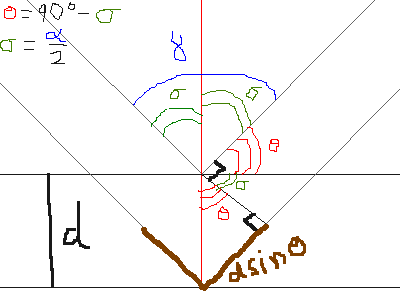
\includegraphics[width=10cm]{images/Derivation}

Since certain crystals' regular atomic structure provides consistently, tightly-packed planes, crystals provide an apparatus for measuring the diffraction of high-frequency waves. Lithium Fluoride is one such crystal. It has a cubic crystal structure and a known density, so the spacing can be computed.

\begin{align*}
MolecularMass_{LiF} & = & AtomicMass_{Li} + AtomicMass_{F} \\
                     & = & 1.15258\e{-23} g + 3.154759\e{-23} g \\
                     & = & 4.307339 \e{-23} g 
\end{align*}

$Density_{LiF} = 2.635 g / cm^3. $

and because it is a cubic structure where the volume of lithium cubes and fluorine cubes is the same, we can say that...

\begin{align*}
2 d^3  & = & Volume_{LiCube} + Volume_{FCube} \\    
d & = & \frac{1}{\sqrt[3]{2}} \sqrt[3]{MolecularMass_{LiF} / Density_{LiF}} \\
d & = & \frac{1}{\sqrt[3]{2}} \sqrt[3]{4.307339\e{-23} g / (2.635 g / cm^3)} \\
d &= 2.014\e{-10}m
\end{align*}

In this experiment, X-Rays are generated by applying a high voltage field to a sheet of copper. The electrons in the current collide with copper's electrons, causing them to jump to higher energy (higher n) shells. One of copper's electrons, then, falls down into the vacated location and release energy as electromagnetic radiation. There are a discrete number of transitions that can take place. The function that describes the maximum number of electrons at any energy level in an atom is $amount(n) = 2n^2.$, so the number of energy levels is the lowest value of n for which this inequality is true: 

$ 2 \sum_{i=1}^{n} i^2 > Z $

Copper, assuming no ionization, has twenty nine electrons, so the smallest n that satisfies that inequality is 4. The set of energy transitions that could result in light emission is, then, \{$E_4 -> E_3, E_4 -> E_2, E_4 -> E_1, E_3 -> E_2, E_3 -> E_1, E_2 -> E_1$\}. With the Bohr model's allowed-energies equation, $E_n = -Z^2E_0 / n^2$ we can compute those energy values. In making those predictions, we will modify the equation to $E_n = -(Z-1)^2E_0 / n^2$ because the other electron in the n=1 shell lowers the strength of the net charge of the center of the atom. Since other transitions involve passing other electrons, that approximation breaks down. With the relationship between the energy and wavelength of light, $E = hc/\lambda$ we can find the total set of allowed wavelengths:

\begin{align*}
E_2 - E_1 &= -(Z - 1)^2 E_0 ( 1/2^2 - 1/1^2) \\
E_2 - E_1 &= -28^2 * 13.6eV * -0.75 \\
E_2 - E_1 &= 7996.8 eV
\end{align*}

\begin{align*}
\lambda_{2-1} &= hc / (E_2 - E_1) \\
\lambda_{2-1} &= 1.2398 eVm\e{-6} / 7996.8 eV \\
\lambda_{2-1} &= 1.5504\e{-10} m
\end{align*}

An apparatus may or may not create a sufficient voltage field to provide the required energy to create shifts from n=2 to n=1. Our apparatus, with options of 20kV or 30 kV, can produce that wavelength because the energy barrier, 7996.8 eV, is less than 20000 eV. 

Since the condition for purely constructive interference of the X-rays is $2d sin(\theta) = n \lambda$, there will be intensity maxima for certain values of n and $\lambda$. Those wavelengths will be among the six possible wavelengths and the 'n' values will most likely be smaller 'n' because diffraction intensity decreases as n increases. This statement requires that d is a constant. From the density derivation, this requirement is met. 

In addition to the electromagnetic emission from energy level shifts, there will be electromagnetic emission from the acceleration of the current around the copper nuclei. The energy loss accompanying this acceleration depends on the distance of the moving electron from the nucleus, so the non-discrete set of distances makes for a continuous distribution of bremmstrahlung emission:

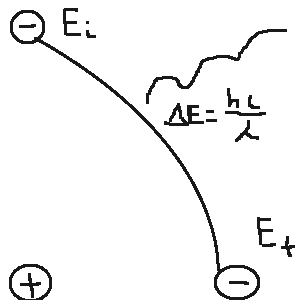
\includegraphics[width=5cm]{images/Brem}

\begin{center} Apparatus and Procedure \end{center}

A copper sheet is placed in an electrical circuit of either 20kV or 30kV. X-rays are emitted, some due to the bremmstrahlung effect and others due to the energy level shifts. These X-rays hit a crystal, LiF, and diffract. There is a detector that takes a circular path around the crystal at constant velocity so that it can compare the intensity of the X-rays at various angles. The angle, $\phi$ on the diagram is the angle at which the detector logs its counts.

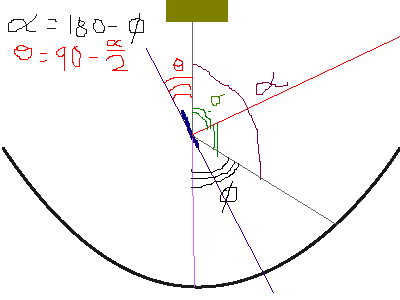
\includegraphics[width=10cm]{images/Apparatus}

Some wide swaths with at 0.2 seconds per step:

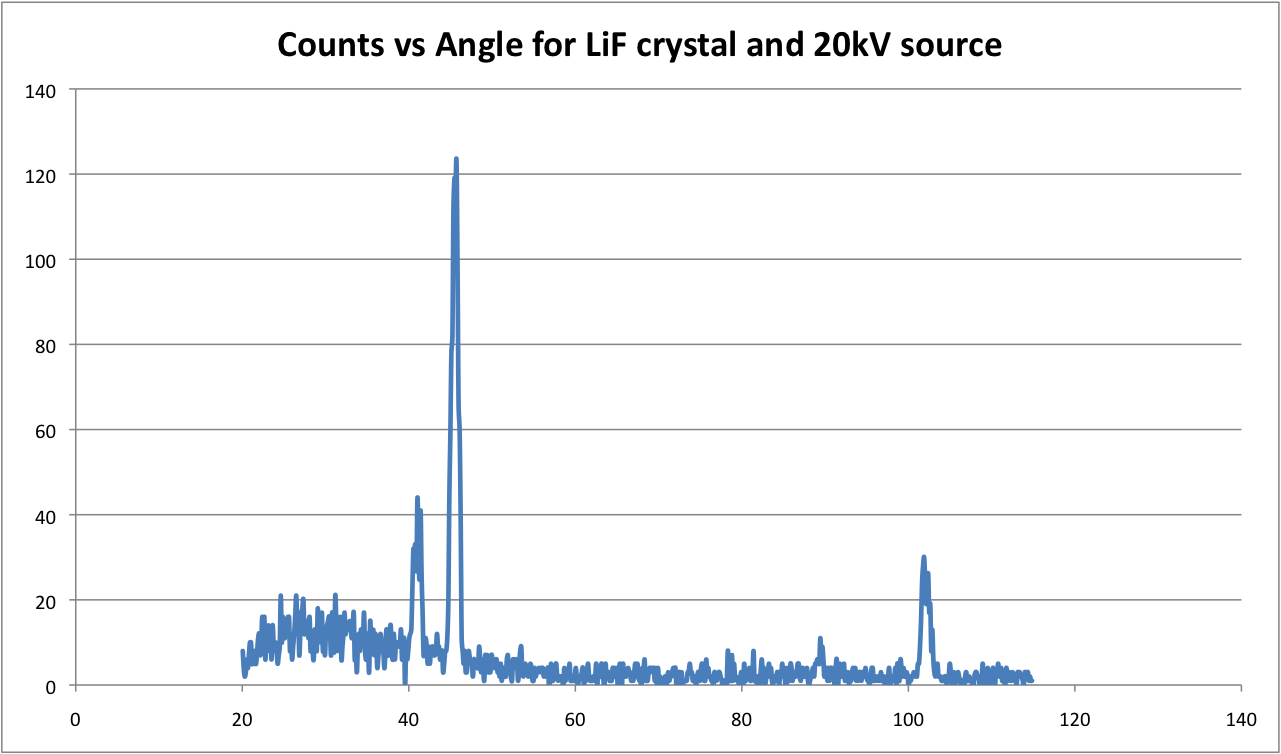
\includegraphics[width=10cm]{images/LiF20kV}

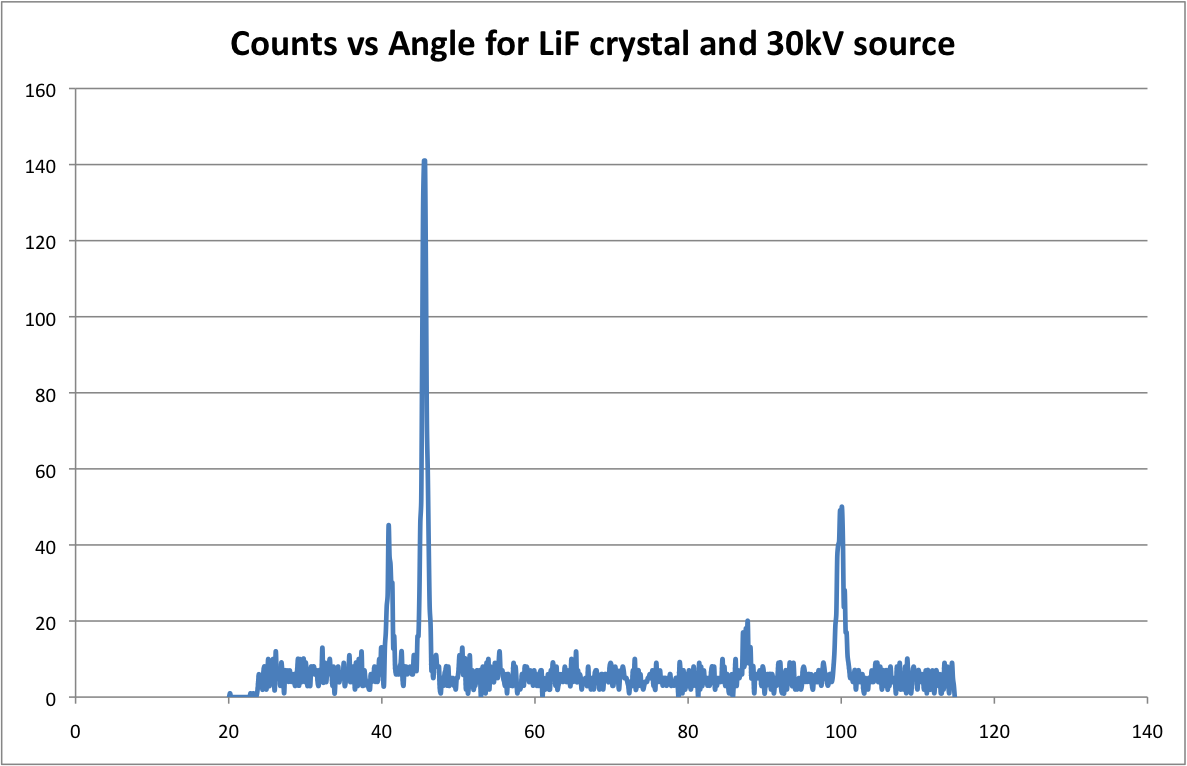
\includegraphics[width=10cm]{images/LiF30kV}


After identifying roughly identifying peaks, we took more time intensive, and thus more accurate, measurements around those maxima.

Because signal noise and background radiation are present, there is a question of whether or not a local maximum value corresponds to an actual maximum. Our method for resolving that question is by trusting our eyes to identify proper peaks by their sufficiently pronounced height and sufficiently long horizontal width. Due to that signal noise, there is also a question of what point exactly is the maximum. We measure that point as the one with the largest count number. Supposing that perfect measurements of the peaks would be symmetrical, we consider the uncertainty in angle measurement to be the difference between the angle of maximum count and the angle at the center of the peak.  

With this method, we measured:

\begin{tabular}{| l | l | l | l | l | l |}
\hline
20kV $\phi$ & uncertainty & counts & 30kV $\phi$ & uncertainty & counts \\
\hline
42.338 & 0.124 & 171 & 33.072 & 0.623 & 44 \\
\hline
47.029 & 0.061 & 497 & 45.025 & 0.061 & 664 \\
\hline
& & & 79.188 & 0.499 & 29 \\
\hline
104.299 & 0.123 & 123 & 94.394 & 0.124 & 62 \\
\hline
\end{tabular}

Due to calibration issues, though, these values are faulty. Rather than using this theoretically better method of time-intensive counting around the maxima and defining uncertainty as the distance between the center of the peak and the measurement of the peak, we use maxima from the lower precision (but higher accuracy) measurements of the whole range. These measurements are the two in this lab report's graphs. Since the lower number of data points in our new dataset makes it difficult to distinguish between the center of the peak and the point of maximum counts, the uncertainty is angle is now defined as the change in angle in two measurement steps.

\begin{tabular}{| l | l | l | l | l | l |}
\hline
20kV $\phi$ & uncertainty & counts & 30kV $\phi$ & uncertainty & counts \\
\hline
41.042 & 0.248 & 44 & 40.883 & 0.248 & 45 \\
\hline
45.733 & 0.248 & 119 & 45.513 & 0.248 & 141 \\
\hline
89.426 & 0.248 & 11 & 87.787 & 0.248 & 20 \\
\hline
101.893 & 0.248 & 30 & 100.091 & 0.248 & 50 \\
\hline
\end{tabular}

\begin{tabular}{| l | l | l | l | l | l |}
\hline
20kV $\theta$ & uncertainty & 30kV $\theta$ & uncertainty \\
\hline
20.251 & 0.124  & 20.442 & 0.124  \\
\hline
22.867 & 0.124  & 22.757 & 0.124  \\
\hline
44.713 & 0.124  & 43.896 & 0.124  \\
\hline
50.947 & 0.124  & 50.050 & 0.124  \\
\hline
\end{tabular}

This table is a simple transformation of the actual measurement table. $\theta = 90 - (180 - \phi) / 2$ or more simply $\theta = \phi / 2$. Since the use of uncertainty is as a proportion of the measurement, the definition of uncertainty in $\theta$ is half of the uncertainty in $\phi$.

\begin{center} Analysis \end{center}


According to the Duana-Hunt rule, there is supposed to be a definite cutoff wavelength at which the continuous distribution stops. That cutoff wavelength is given by $\lambda_m = 1240 nm / V$. The theoretical values for our experimental voltages, 20kV and 30kV, would be $6.2\e{-11} m$ and $4.13\e{-11} m$. Using the diffraction equation like so:  

\begin{align*}
\theta &= arcsin(n \lambda / 2 d) \\
\theta &= arcsin(1 * 6.2\e{-11} m / 2 * 2.014\e{-10} m) \\
\theta &= 8.854 \text{ degrees} \\
\phi &= 2 \theta \\
\phi &= 17.709 \text{ degrees} 
\end{align*}

we can calculate the cutoff angle table:
\begin{tabular}{| l | l | l |}
\hline
 $\phi$ & $\lambda_{20kV}$ & $\lambda_{30kV}$ \\
\hline
n & 6.2\e{-11} m & 4.13\e{-11} m \\
\hline
1 & 17.709 & 11.770 \\
\hline
2 & 35.859 & 23.670 \\
\hline
3 & 55.002 & 35.829 \\
\hline
\end{tabular}

Mode 1 of the bremmstrahlung cutoff are not observable in our $20 <= \phi <= 115$ measurement. The mode 2 cutoffs are notably observable on the graph. Intensity decreases with mode, so the mode 3 cutoff angle is not significally visible.

While the bremmstrahlung effect should vary based on the input voltage, the location of the peaks should not. This invariance is due to the maxima corresponding to discrete energy level shifts in copper. The presence of the peaks can change, depending on whether the current has sufficient potential to create the peak's corresponding energy level transition. Although the approximation  $E = -(Z-1)^2 E_0 (1/n^2 - 1)$ breaks down for high n due to the effects of electrons, the effect of those electrons is to decrease the value of the potential difference, so that approximation provides an upper bound for copper's actual energy level shifts (whose computation is much more complicated). Since copper's largest energy energy level difference is from n=4 to n=1: 

\begin{align*}
E_4 - E_1 &= -(29 - 1)^2 13.6 eV ( 1/4^2 - 1/1^2) \\
E_4 - E_1 &= 9996.0 eV
\end{align*}

This value is less than 20keV, so the current's voltage should have no presence on the presence of intensity maxima.  Three of the four 20kv,30kV peak pairs are equal to each other within uncertainty and the fourth is nearly within uncertainty.  The intensity at the peaks, however, increased from the 20kV trial to the 30kV trial. The physical explanation for this is that a higher-voltage current running through the source causes energy level shifts of the same type to occur more frequently. 


With the wavelength calculated from the $E = -(Z-1)^2 E_0 (1/n^2 - 1)$ approximation and the lattice plane spacing calculated from the molecular mass and density, we can apply the $ 2d sin(theta) = n \lambda $ equation to predict the $\theta$ that we also measured with our apparatus. For n=1, $\theta = 22.638$ degrees and for n=2, $\theta = 50.337$ degrees. That prediction for n=1 is accurate to the 30kV experimental value, $\theta = 22.757$ degrees, within uncertainty; it is 1.85 margins of error less than the 20kV experimental value, $\theta =  22.867$ degrees. That prediction for n=2 is 2.3 margins of error greater than the 30kV experimental value; it is 4.9 margins of error less than the 20kV experimental value. This is a low-quality agreement between theory and experiment, but those experimental values can probably be explained as modes 1 and 2 of the $shell_2$ to $shell_1$ electron transition's x-ray emission. The other experimental peaks, at $\theta = 20.251$ degrees and $\theta = 44.713$ degrees are probably due to another shell transition whose energy is complicated to predict.

Since the experimental angle is equal to the theoretical angle due to mode 1 of the $shell_2$ to $shell_1$ transition within uncertainty, we can use the experimental angle with the theoretical mode and wavelength to compute 'd'. Of course, this equality within uncertainty could be entirely coincidental but I will assume that $n=1 and \lambda = 1.5504\e{-10}$ is the physical explanation for the presence of an intensity maximum at $\theta = 22.757$ degrees.

\begin{align*}
\ 2d sin(\theta) &= n \lambda \\
\ d &= \frac{1 * 1.5504\e{-10} m}{2 * sin(22.757)} \\
\ d &= 2.0040 m 
\end{align*}

\begin{align*}
\ 2 d_{hi} sin(\theta - uncertainty) &= n \lambda \\
\ d_{hi} &= \frac{1 * 1.5504\e{-10} m}{2 * sin(22.757 - 0.124)} \\
\ d_{hi} &= 2.0144 m 
\end{align*}

That range includes the value for d computed in the 'theory' section, $2.014\e{1-}$, so our prediction of d is precise within uncertainty. 
\end{document}
